% CVPR 2023 Paper Template
% based on the CVPR template provided by Ming-Ming Cheng (https://github.com/MCG-NKU/CVPR_Template)
% modified and extended by Stefan Roth (stefan.roth@NOSPAMtu-darmstadt.de)

\documentclass[10pt,twocolumn,letterpaper]{article}

%%%%%%%%% PAPER TYPE  - PLEASE UPDATE FOR FINAL VERSION
% \usepackage[review]{cvpr}      % To produce the REVIEW version
% \usepackage{cvpr}              % To produce the CAMERA-READY version
\usepackage[pagenumbers]{cvpr} % To force page numbers, e.g. for an arXiv version

% Include other packages here, before hyperref.
\usepackage{graphicx}
\usepackage{amsmath}
\usepackage{amssymb}
\usepackage{booktabs}
\usepackage{cite}


% It is strongly recommended to use hyperref, especially for the review version.
% hyperref with option pagebackref eases the reviewers' job.
% Please disable hyperref *only* if you encounter grave issues, e.g. with the
% file validation for the camera-ready version.
%
% If you comment hyperref and then uncomment it, you should delete
% ReviewTempalte.aux before re-running LaTeX.
% (Or just hit 'q' on the first LaTeX run, let it finish, and you
%  should be clear).
\usepackage[pagebackref,breaklinks,colorlinks]{hyperref}


% Support for easy cross-referencing
\usepackage[capitalize]{cleveref}
\crefname{section}{Sec.}{Secs.}
\Crefname{section}{Section}{Sections}
\Crefname{table}{Table}{Tables}
\crefname{table}{Tab.}{Tabs.}


%%%%%%%%% PAPER ID  - PLEASE UPDATE
\def\cvprPaperID{*****} % *** Enter the CVPR Paper ID here
\def\confName{CVPR}
\def\confYear{2023}


\begin{document}

%%%%%%%%% TITLE - PLEASE UPDATE
% \title{\LaTeX\ Author Guidelines for \confName~Proceedings}
\title{SimTrans: A Self-supervised Method for Biomedical Image Segmentation}

\author{Shengfan Wang\\
CSBIO\\
SEIEE 2-306\\
{\tt\small diofan0814@sjtu.edu.cn}
% For a paper whose authors are all at the same institution,
% omit the following lines up until the closing ``}''.
% Additional authors and addresses can be added with ``\and'',
% just like the second author.
% To save space, use either the email address or home page, not both
\and
Zhen Zhou\\
CSBIO\\
SEIEE 2-306\\
{\tt\small zz20020101@sjtu.edu.cn}
\and
Jiabei Cheng\\
CSBIO\\
SEIEE 2-306\\
{\tt\small jiabei\_cheng@sjtu.edu.cn}
\and
Changyong Li\\
CSBIO\\
SEIEE 2-306\\
{\tt\small steven\_li@sjtu.edu.cn}
}
\maketitle

%%%%%%%%% ABSTRACT
\begin{abstract}
   The ABSTRACT is to be in fully justified italicized text, at the top of the left-hand column, below the author and affiliation information.
   Use the word ``Abstract'' as the title, in 12-point Times, boldface type, centered relative to the column, initially capitalized.
   The abstract is to be in 10-point, single-spaced type.
   Leave two blank lines after the Abstract, then begin the main text.
   Look at previous CVPR abstracts to get a feel for style and length.
\end{abstract}

%%%%%%%%% BODY TEXT
\section{Introduction}
\label{sec:intro}

With the rapid development of deep learning technology, many fields have started to adopt deep learning techniques to improve task efficiency. Training deep learning models requires a large amount of data, and this data needs to have corresponding labels in order to train models that have strong fitting and generalization capabilities. However, in the field of biomedical imaging, it is not possible to obtain a large amount of data due to patient privacy concerns. Additionally, the annotation of biomedical images requires professional medical experts, which further increases the cost of data annotation. As a result, there is a scarcity of biomedical imaging datasets, and the number of annotated data samples is even smaller.
Biomedical image segmentation typically involves pixel-level classification of lesions, tissues, and organs in biomedical images. These lesions, tissues, and organs generally occupy a large space or are far apart in biomedical images. Based on this characteristic, we analyzed the current mainstream biomedical image segmentation models based on convolutional neural networks (CNNs). These models use traditional convolutional approaches for feature extraction. However, traditional convolutions are limited by their receptive field and can only extract local features of the target, failing to capture global features. This can cause the model to struggle in distinguishing background regions in the image and may misclassify background pixels as the features of interest, leading to a decrease in segmentation accuracy. Researchers have proposed various methods to address these issues, such as using multiple convolutional kernels of different sizes or downsampling to reduce image resolution. These methods partially solve the problem of CNNs' inability to capture global features. However, they either increase the model's complexity and reduce its runtime speed or sacrifice some local feature information, resulting in a decrease in model accuracy without achieving a balance.
To address the aforementioned problems, this paper proposes an end-to-end deep learning network based on self-supervised learning. In this approach, the self-supervised framework SimCLR is first employed for training, overcoming the lack of labeled data by directly extracting the data distribution features. Then, the encoder part of SimCLR, which captures the data distribution, is separated and combined with a decoder to accomplish the downstream end-to-end segmentation task. This method is named SimTrans, derived from the combination of the self-supervised framework SimCLR and the Transformer framework.
The paper begins by introducing the self-supervised learning framework SimCLR, followed by an introduction to the Swin Transformer framework. It then presents the weighted structured loss function used for the downstream task and introduces the proposed SimTrans deep learning framework. Finally, the paper conducts experiments to evaluate the proposed model, providing details on the experimental setup, results, and analysis.

%------------------------------------------------------------------------
\section{Related Work}
\label{sec:related work}

\subsection{SimCLR}

To address the scarcity of biomedical image datasets, researchers aim to develop models that can learn features directly from the data without the need for labeled data. This approach, known as self-supervised learning, allows models to learn features from the data itself. One widely studied self-supervised learning framework in the field is SimCLR\cite{SimCLR}, proposed by Hinton et al.
SimCLR consists of four main components: data augmentation, a base encoder, a projection head, and a contrastive loss. The framework is designed to learn powerful representations from unlabeled data. In SimCLR, data augmentation is applied to generate multiple augmented versions of each unlabeled sample. These augmented samples are then passed through the base encoder, which extracts their features. The projection head further processes the encoded features to produce informative representations. Finally, the contrastive loss function encourages similar representations of augmented samples from the same sample while pushing representations from different samples apart.

\begin{figure}[htbp]   %注意,这里设置是关键
	\centering
	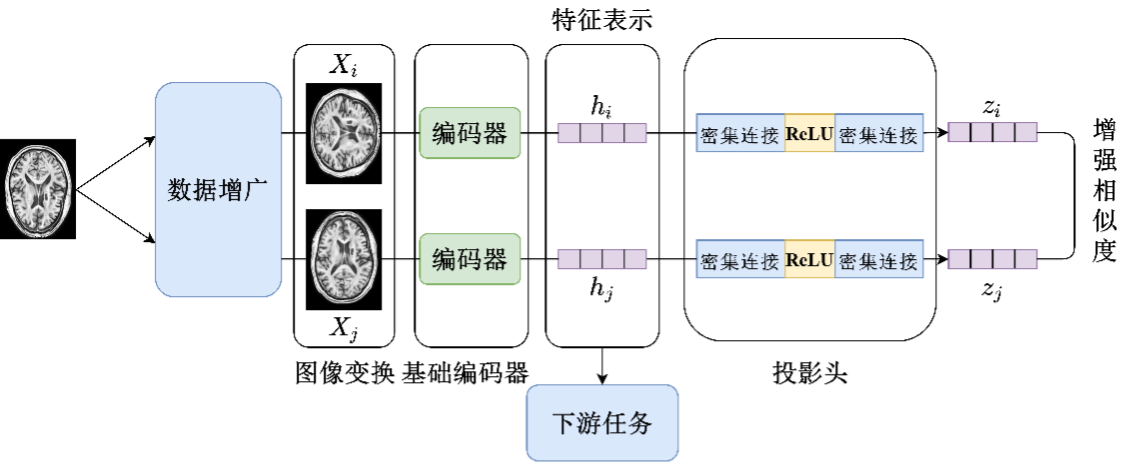
\includegraphics[width=\linewidth,scale=1.00]{Images/SimCLR.png}
	\caption{Framwork of SimCLR.}
	\label{fig:simclr}
\end{figure}

The overall objective of SimCLR is to maximize agreement between differently augmented views of the same data sample while minimizing agreement between different samples. This enables the model to learn rich and discriminative representations without the need for explicit labels. SimCLR has garnered significant attention from researchers and has achieved remarkable results in various computer vision tasks, including biomedical image analysis.

The data augmentation module in SimCLR performs random transformations on given data samples to generate two correlated views of the same sample, denoted as $x_i$ and $x_j$. These two views are treated as a positive sample pair. Data augmentation techniques used in SimCLR include random cropping, resizing, color distortion, and Gaussian blur. These operations generate pseudo-labels, which are then utilized to train the model.
The encoder in SimCLR extracts feature vectors, represented as $h_i$ and $h_j$, from the augmented data samples. The choice of encoder is not constrained and commonly used backbone frameworks like VGG and ResNet can serve as encoders in SimCLR.
The projection head maps the data representations to the space of contrastive loss. A common approach is to use a single-layer multilayer perceptron (MLP) for this mapping, as shown in Equation (1):

\begin{equation}
z_i=g\left(h_i\right)=W^{(2)} \sigma\left(W^{(2)} h_i\right)
\end{equation}

Here, $g(\cdot)$ represents the mapping function,  $\sigma$ is the ReLU activation function. According to the experimental analysis by the authors of SimCLR, defining the contrastive loss on the projected feature representation $z_i$ tends to yield better results compared to using the feature representation $h_i$ directly from the encoder.
The contrastive loss module defines the contrastive loss function for the contrastive prediction task. The key component of SimCLR is the normalized temperature-scaled cross-entropy loss (NT-Xent) used as the contrastive loss, given by Equation (2):

\begin{equation}
  \ell_{i, j}=-\log \frac{\exp \left(\operatorname{sim}\left(z_i, z_j\right) / \tau\right)}{\sum_{k=1}^{2 N} \mathbb{1}_{[k \neq i]} \exp \left(\operatorname{sim}\left(z_i, z_k\right) / \tau\right)}
\end{equation}
First, it calculates the similarity between a positive pair and all negative representations. The cosine similarity function is commonly used as a distance metric. Then, negative cross-entropy loss is employed to calculate the loss function for the positive sample pair $(i, j)$.

%------------------------------------------------------------------------


\subsection{Swin Transformer}

Swin Transformer\cite{ST} is a hierarchical structure that builds feature maps by merging image patches at deeper layers, allowing flexible modeling at multiple scales. It achieves a linear computational complexity relative to the image size by computing self-attention within each local non-overlapping window. Additionally, Swin Transformer enables cross-window connections, as shown in Figure 2. The self-attention computation of a new window spans the boundaries of previously processed windows in layer $l$, providing cross-window connections between adjacent non-overlapping windows. This operation has been found effective in tasks such as image classification, object detection, and semantic segmentation. The ability to model visual entities of various scales and replace quadratic complexity with linear computational complexity contributes to Swin Transformer's versatility as a backbone for various visual tasks.

\begin{figure}[htbp]   %注意,这里设置是关键
	\centering
	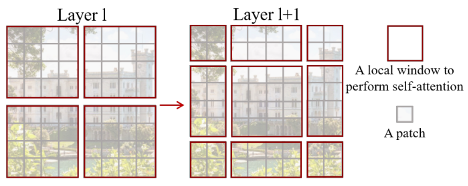
\includegraphics[width=\linewidth,scale=1.00]{Images/ST_1.png}
	\caption{Self-attention computation for non-overlapping windows.}
	\label{fig:st_1}
\end{figure}

Swin Transformer consists of a Multi-head Self-Attention module (MSA) based on movable windows, followed by a two-layer Multilayer Perceptron (MLP) with Gaussian Error Linear Units (GELU) as the non-linear activation function. GELU is a high-performance neural network activation function that weights the inputs rather than gating them with signs as in ReLU. Layer Normalization (LN) is applied before each MSA module and each MLP, and a residual connection is employed after each module, as shown in Figure 3.
The computational complexity of the standalone MSA module in Swin Transformer has a quadratic relationship with the image size, as shown in Equation (3):


\begin{equation}
  \Omega(M S A)=4 h w C^2+2(h w)^2 C
\end{equation}

However, in Swin Transformer, the self-attention computation is performed within non-overlapping local windows, resulting in a linear computational complexity relative to the image size, as shown in Equation (4):

\begin{equation}
  \Omega(W-M S A)=4 h w C^2+2 M^2 h w C
\end{equation}

Here, $M$ is a constant.
Furthermore, Swin Transformer incorporates relative position information into the attention computation, as shown in Equation (5):

\begin{equation}
  \operatorname{Attention}(Q, K, V)=\operatorname{SoftMax}\left(\frac{Q K^T}{\sqrt{d}}+B\right) V
\end{equation}

Where $Q$, $K$, and $V$ represent the query matrix, key matrix, and value matrix, respectively. $d$ is the dimension, and $B$ represents the relative position bias. Compared to using absolute positions, incorporating relative positional biases significantly improves the model's performance.
Additionally, Swin Transformer introduces inductive biases such as locality, hierarchical feature representation, and translation equivariance, enabling it to serve as a universal backbone network for various image recognition tasks.

\begin{figure}[htbp]   %注意,这里设置是关键
	\centering
	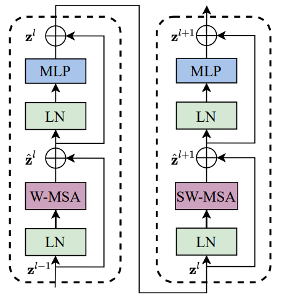
\includegraphics[width=0.8\linewidth,scale=1.00]{Images/ST_2.png}
	\caption{Block of Swin Transformer.}
	\label{fig:st_2}
\end{figure}

%------------------------------------------------------------------------

\subsection{Residual Channel Attention}

The Residual Channel Attention (RCA)\cite{RCAB} module combines channel attention and residual connections. By using channel attention, it can capture features from different channels and enhance channel-wise information. The residual connections then connect the features, allowing for more refined feature representation. The structure of the RCA module is illustrated in Figure 5.

\begin{figure}[htbp]   %注意,这里设置是关键
	\centering
	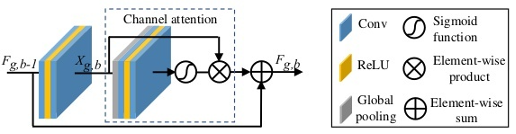
\includegraphics[width=\linewidth,scale=1.00]{Images/RCBA.png}
	\caption{Structure of RCBA.}
	\label{fig:rcba}
\end{figure}

%------------------------------------------------------------------------

\subsection{Multi-scale Dilated Convolution}

Multi-scale dilated convolution\cite{MSD} is composed of convolutions with different dilation rates. Firstly, the feature map undergoes multiple convolution layers with different dilation rates. Then, the output results from each convolution layer are cascaded together to form the output of the entire module. This approach not only addresses the issue of information discontinuity caused by dilation but also helps the model capture multi-scale feature information. Figure 6 illustrates dilated convolutions, with the left side showing a dilated convolution with a dilation rate of 2, and the right side showing a dilated convolution with a dilation rate of 3.

\begin{figure}[htbp]   %注意,这里设置是关键
	\centering
	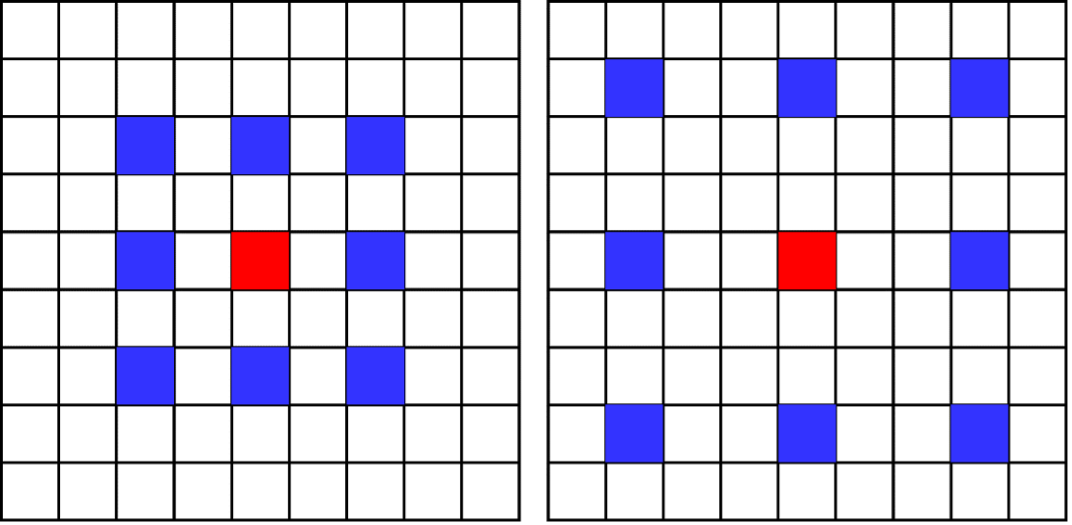
\includegraphics[width=\linewidth,scale=1.00]{Images/MSD.png}
	\caption{Structure of MSD.}
	\label{fig:msd}
\end{figure}

%------------------------------------------------------------------------

\section{Method}
\label{sec:method}

We utilize Swin Transformer as the encoder in the SimCLR framework and train it using unlabeled data, allowing the Swin Transformer to learn the distribution and features of the data with the help of pseudo-labels. Then, we apply the learned feature encoder to downstream segmentation tasks. Based on SimCLR and Swin Transformer, we design a deep learning network model called SimTrans, as shown in Figure 4. In the downstream tasks, to achieve an end-to-end output, a simple decoder is employed. It fuses the features obtained at different stages of the Swin Transformer and includes a decoder module that upsamples the fused features for comparison with the label map. Additionally, to better train the model, we propose a weighted structured loss function based on existing loss functions. It is a weighted sum of binary cross-entropy loss (BCE) and intersection over union loss (IOU):

\begin{equation}
  L(s, y)=w * L_{b c e}(s, y)+L_{i o u}(s, y)
\end{equation}

Here, $Y$ represents the label, $W$ represents the edge weight $w=1+5 *|(a p(x)-y)|)$, $\quad a p(\cdot)$ represents the average pooling operation.

\begin{figure}[htbp]   %注意,这里设置是关键
	\centering
	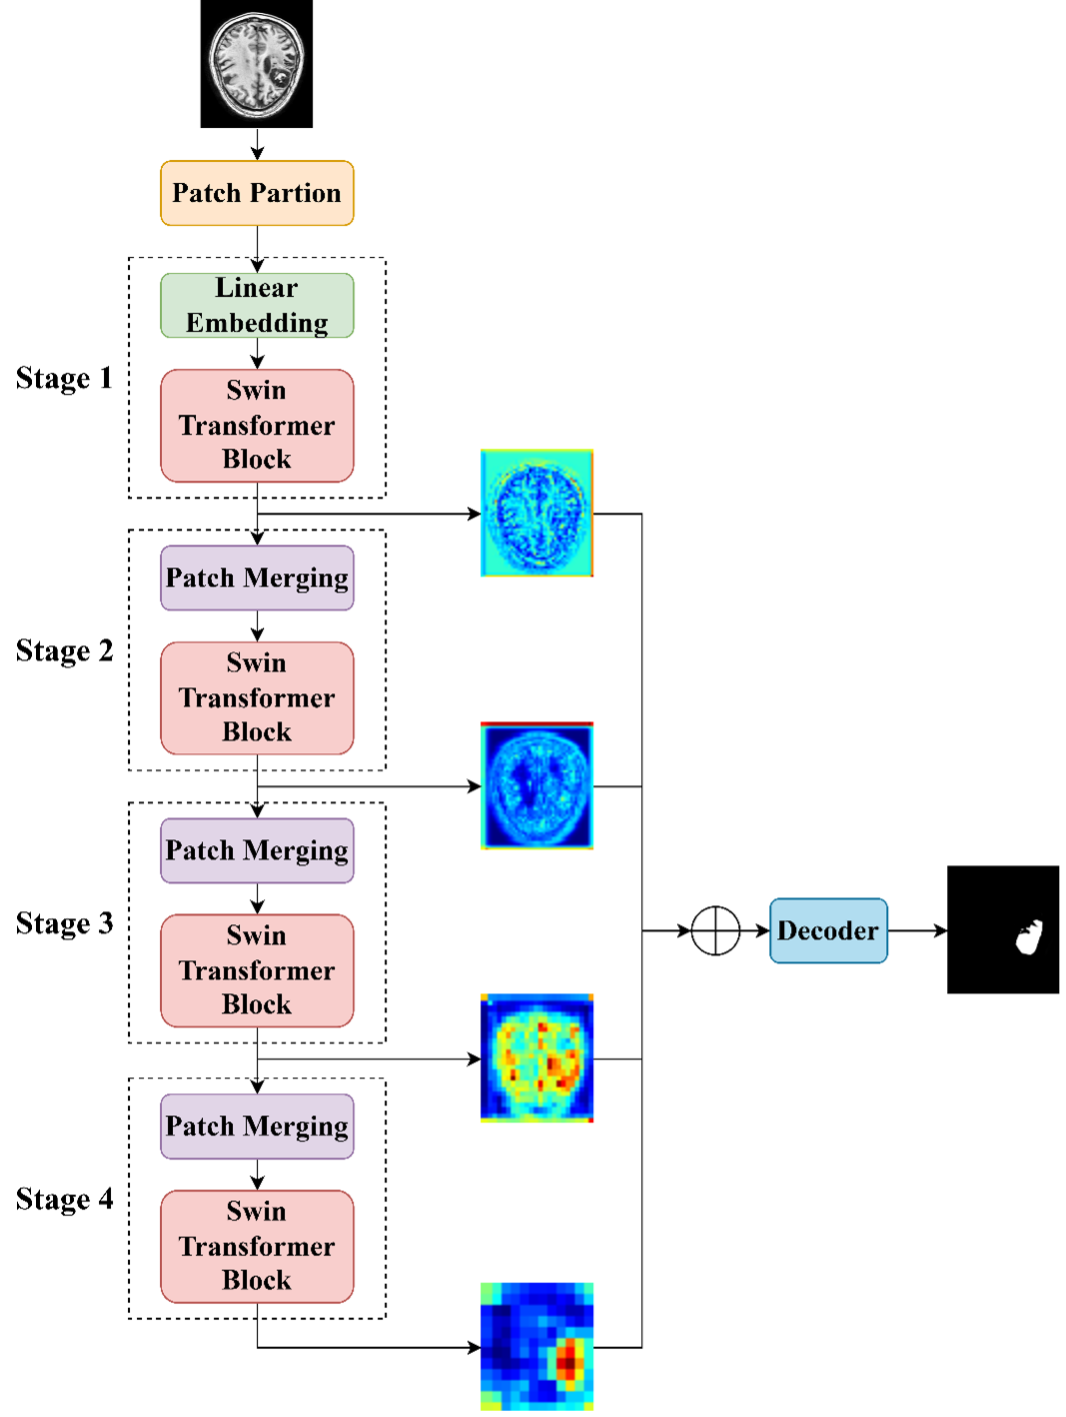
\includegraphics[width=\linewidth,scale=1.00]{Images/SimTrans.png}
	\caption{Structure of SimTrans.}
	\label{fig:simtrans}
\end{figure}

The SimTrans model is based on the self-supervised learning framework SimCLR and the Transformer model, specifically designed for the challenges of biomedical image datasets with limited annotated data. This model leverages the strategy of SimCLR, which involves data augmentation techniques to generate multiple augmented images from a single image. These generated images serve as positive examples, while the other images in a training batch act as negative examples. This allows for the reduction of the distance between positive examples and the separation of negative examples.
After deciding to use the self-supervised learning framework of SimCLR, we compared various commonly used backbone architectures such as VGG and ResNet. However, these architectures, based on traditional convolutional neural networks, have certain limitations, such as fixed receptive fields and large model sizes. Considering the need for global feature consideration in biomedical images, a model capable of capturing long-range dependencies was preferred. Therefore, the Transformer framework was considered, and different Transformer architectures such as ViT and TransUNet were evaluated. Ultimately, Swin Transformer was selected due to its ability to capture global features using the Transformer's long-range dependency modeling capabilities. Additionally, the introduction of a sliding window approach for attention computation in Swin Transformer reduced the number of parameters required for global attention computation. Moreover, Swin Transformer has a hierarchical design that continuously reduces the resolution of input feature maps, similar to the downsampling process in convolutional neural networks, to expand the receptive field.
Using Swin Transformer as the encoder part of SimCLR, training is conducted using generated pseudo-labels. Once training is completed, for the downstream task of biomedical image segmentation, a decoder is added to Swin Transformer. The decoder consists of two modules: Residual Channel Attention Block (RCAB) and Multi-Scale Dilated Convolution (MSD).

%------------------------------------------------------------------------

\section{Experiment}
\label{sec:experiment}

This study conducted experimental validation of the proposed deep learning model on the ATLAS (Automatic Labeling of Brain Stroke Lesion) dataset\cite{ATLAS}, which is a publicly available dataset for brain stroke lesion segmentation. The dataset consists of a total of 229 T1-weighted brain magnetic resonance imaging (MRI) images provided by 11 different medical research centers. These images are expertly annotated by professional physicians. Each three-dimensional image has a voxel size of 0.9mm $\times$ 0.9mm $\times$ 0.3mm and contains 189 slices. Each slice has dimensions of 233 $\times$ 197. The entire ATLAS dataset consists of 43,281 two-dimensional slices. In this study, 10,203 labeled data were processed and used for validation in the downstream segmentation task, while the remaining 33,078 slices were used for self-supervised learning to learn the features of brain stroke data.
Three evaluation metrics, namely Dice coefficient, mean intersection over union (IoU), and precision, were selected to quantify the performance of the proposed model.
All the experiments were conducted in the PyTorch framework and trained using Nvidia-RTX 3090Ti GPUs. The deep learning models were trained for a total of 50 epochs.

\subsection{Results and Analysis}

This study employed the self-supervised learning framework SimCLR to learn the features of unlabeled data. SimCLR utilizes data augmentation techniques to generate pseudo-labels, as shown in Figure 7.

\begin{figure}[htbp]   %注意,这里设置是关键
	\centering
	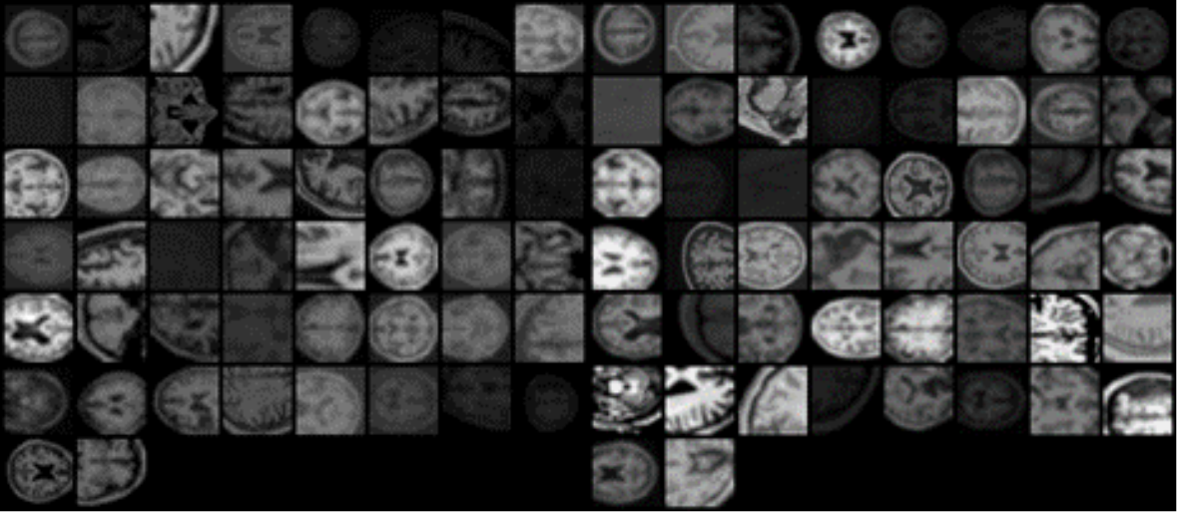
\includegraphics[width=\linewidth,scale=1.00]{Images/DR_SimCLR.png}
	\caption{Different representations of the same image produced by SimCLR.}
  \label{fig:dr_simclr}
\end{figure}

To assess whether the SimTrans model focuses more on the lesion regions at different stages, the feature maps were visualized and analyzed. Figure 8 illustrates the visualization of the feature maps.

\begin{figure}[htbp]   %注意,这里设置是关键
	\centering
	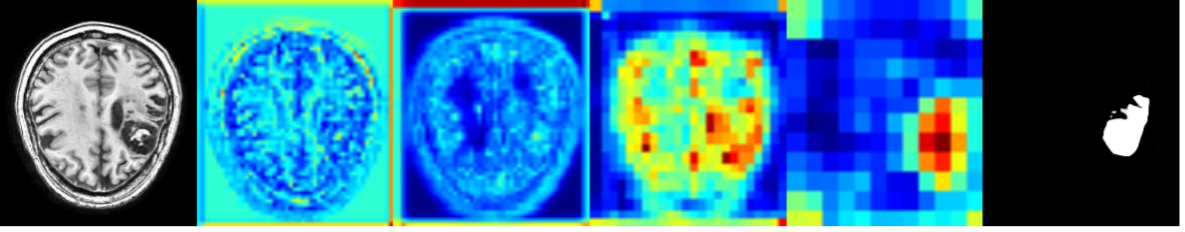
\includegraphics[width=\linewidth,scale=1.00]{Images/Vision.png}
	\caption{Feature visualization.}
  \label{fig:vision}
\end{figure}

Figure 8 displays the following images from left to right: the original brain MRI image, feature maps from the first stage, feature maps from the second stage, feature maps from the third stage, feature maps from the fourth stage, and the ground truth label map. From the visualization, it can be observed that the SimTrans model progressively increases its attention to the lesion regions, demonstrating its effectiveness in segmenting the target regions.
The comparison results between SimTrans and two other networks, ResUNet\cite(ResUNet) and ViT\cite{ViT}, are presented in Table 1.

\begin{table}
  \centering
  \begin{tabular}{lccc}
    \toprule
    Model & Dice & MIoU & Precision \\
    \midrule
    ResUNet & 0.6810 & 0.5552 & 0.5583 \\
    ViT & 0.6783 & 0.5496 & 0.5529 \\
    SimTrans & 0.7585 & 0.6424 & 0.6453 \\
    \bottomrule
  \end{tabular}
  \caption{Segmentation results comparison.}
  \label{tab:result_1}
\end{table}

It can be observed that when comparing SimTrans with ResUNet, there is an improvement of 0.0775 in Dice coefficient, 0.0872 in Mean Intersection over Union (MIoU), and 0.0870 in precision. These results indicate that the SimTrans network exhibits strong generalization ability and excellent segmentation performance. It can accurately segment the regions affected by brain stroke. The visualization of the segmentation results is shown in Figure 9. From left to right, each column represents the original image, the ground truth label map, the predicted map from ViT, the predicted map from ResUNet, and the predicted map from SimTrans.

\begin{figure}[htbp]   %注意,这里设置是关键
	\centering
	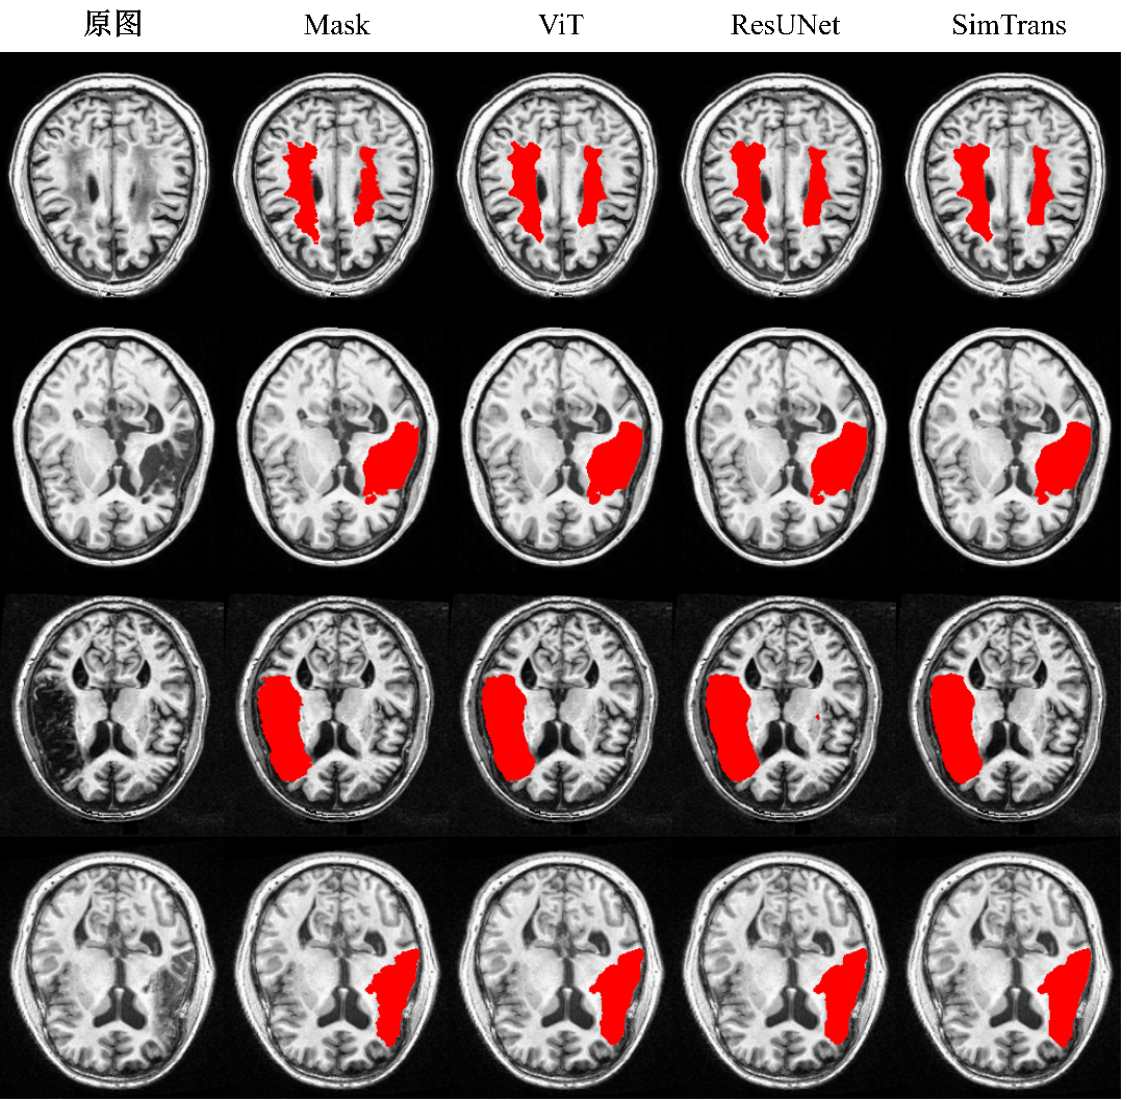
\includegraphics[width=\linewidth,scale=1.00]{Images/Results.png}
	\caption{Model segmentation visualization.}
  \label{fig:result}
\end{figure}

The comparison of parameter count and computational complexity for each model is presented in Table 2. From the table, it can be observed that SimTrans has fewer parameters and lower computational complexity compared to ViT, which is also a Transformer-based model. However, when compared to the classic ResUNet network model, which is based on ResNet as its backbone, there is still some gap. Although SimTrans shows improvement in accuracy, there is still room for progress in terms of model size and computational complexity.

\begin{table}
  \centering
  \begin{tabular}{lccc}
    \toprule
    Metric & ResUNet & ViT & SimTrans \\
    \midrule
    Parameters/MB & 24.01 & 108.25 & 87.32 \\
    Complexity/GMac & 15.24 & 55.42 & 47.51 \\
    \bottomrule
  \end{tabular}
  \caption{Parameter and Computational Complexity comparison.}
  \label{tab:result_2}
\end{table}

%------------------------------------------------------------------------

\section{Conclusion}
\label{sec:conclusion}

This paper proposes an end-to-end self-supervised deep learning network model called SimTrans for the segmentation of brain stroke magnetic resonance imaging (MRI) images. SimTrans utilizes the self-supervised learning framework SimCLR to learn the data distribution and features from unlabeled data. The trained encoder framework, Swin Transformer, is then combined with a decoder structure for the segmentation of brain stroke regions. Additionally, a weighted structured loss function is introduced specifically for brain stroke segmentation to aid the model in achieving better segmentation results. Experimental results on the publicly available brain stroke dataset ATLAS demonstrate the effectiveness of the proposed network model in brain stroke segmentation.

%-------------------------------------------------------------------------
\section{References}
\label{sec:references}

List and number all bibliographical references in 9-point Times, single-spaced, at the end of your paper.
When referenced in the text, enclose the citation number in square brackets, for
example~.
Where appropriate, include page numbers and the name(s) of editors of referenced books.
When you cite multiple papers at once, please make sure that you cite them in numerical order like this.
If you use the template as advised, this will be taken care of automatically.

%-------------------------------------------------------------------------


%%%%%%%%% REFERENCES
{\small
\bibliographystyle{ieee_fullname}
\bibliography{egbib}
}

\end{document}
